\documentclass[11pt]{article}
\usepackage{geometry}
\usepackage[utf8]{inputenc}
\usepackage[english]{babel}
\usepackage{amsmath}
\usepackage{amssymb}
\usepackage{amsfonts}
\usepackage[
    pdftex, 
    dvipsnames
]{xcolor}
\usepackage[
    colorlinks=true,
    linkcolor=black,
    urlcolor=Thistle
]{hyperref}
\usepackage{fancyhdr}
\usepackage{datetime}
\usepackage{xargs}
\usepackage{ccicons}
\usepackage{mdframed}
\usepackage{caption}
\usepackage{cancel}
\usepackage[nottoc]{tocbibind}
\usepackage[
    outputdir=.texpadtmp
]{minted}

% ==== License =====
\usepackage[
    type={CC}, 
    modifier={by-nc-sa}, 
    version={4.0},
]{doclicense}

% ==== todo notes ====
\usepackage[
    colorinlistoftodos,
    prependcaption,
    textsize=tiny
]{todonotes}
\newcommandx{\note}[2][1=]{\todo[linecolor=Thistle,backgroundcolor=Thistle!25,bordercolor=Thistle,#1]{#2}}
\newcommandx{\unsure}[2][1=]{\todo[linecolor=red,backgroundcolor=red!25,bordercolor=red,#1]{#2}}
\newcommandx{\change}[2][1=]{\todo[linecolor=blue,backgroundcolor=blue!25,bordercolor=blue,#1]{#2}}
\newcommandx{\info}[2][1=]{\todo[linecolor=OliveGreen,backgroundcolor=OliveGreen!25,bordercolor=OliveGreen,#1]{#2}}

% General
\newcommand{\mc}[1]{\mathcal{#1}}

% Math Bold Font, Vector Notations
\newcommand{\ba}{\mathbf{a}}
\newcommand{\bb}{\mathbf{b}}
\newcommand{\bc}{\mathbf{c}}
\newcommand{\bd}{\mathbf{d}}
\newcommand{\be}{\mathbf{e}}
\renewcommand{\bf}{\mathbf{f}}
\newcommand{\bg}{\mathbf{g}}
\newcommand{\bh}{\mathbf{h}}
\newcommand{\bi}{\mathbf{i}}
\newcommand{\bj}{\mathbf{j}}
\newcommand{\bk}{\mathbf{k}}
\newcommand{\bl}{\mathbf{l}}
\newcommand{\bm}{\mathbf{m}}
\newcommand{\bn}{\mathbf{n}}
\newcommand{\bo}{\mathbf{o}}
\newcommand{\bp}{\mathbf{p}}
\newcommand{\bq}{\mathbf{q}}
\newcommand{\br}{\mathbf{r}}
\newcommand{\bs}{\mathbf{s}}
\newcommand{\bt}{\mathbf{t}}
\newcommand{\bu}{\mathbf{u}}
\newcommand{\bv}{\mathbf{v}}
\newcommand{\bw}{\mathbf{w}}
\newcommand{\bx}{\mathbf{x}}
\newcommand{\by}{\mathbf{y}}
\newcommand{\bz}{\mathbf{z}}
\newcommand{\bzero}{\mathbf{0}}

% Proofs, Structures
\newcommand{\proof}{\tit{\underline{Proof:}}} % This equivalent to the \begin{proof}\end{proof} block
\newcommand{\proofforward}{\tit{\underline{Proof($\implies$):}}}
\newcommand{\proofback}{\tit{\underline{Proof($\impliedby$):}}}
\newcommand{\proofsuperset}{\tit{\underline{Proof($\supseteq$):}}}
\newcommand{\proofsubset}{\tit{\underline{Proof($\subseteq$):}}}
\newcommand{\contradiction}{$\longrightarrow\!\longleftarrow$}
\newcommand{\qed}{\hfill $\blacksquare$}

% Number Spaces, Vector Space
\newcommand{\R}{\mathbb{R}}
\newcommand{\real}{\mathbb{R}}
\newcommand{\complex}{\mathbb{C}}
\newcommand{\field}{\mathbb{F}}

% customized commands
\newcommand{\settag}[1]{\renewcommand{\theenumi}{#1}}
\newcommand{\tbf}[1]{\textbf{#1}}
\newcommand{\tit}[1]{\textit{#1}}
\newcommand{\overbar}[1]{\mkern 1.5mu\overline{\mkern-1.5mu#1\mkern-1.5mu}\mkern 1.5mu}
\newcommand{\double}[1]{\mathbb{#1}} % Set to behave like that on word
\newcommand{\trans}[3]{$#1:#2\rightarrow{}#3$}
\newcommand{\map}[3]{\text{$\left[#1\right]_{#2}^{#3}$}}
\newcommand{\dime}[1]{\mathrm{dim}(#1)}
\newcommand{\mat}[2]{M_{#1 \times #2}(\R)}
\newcommand{\aug}{\fboxsep=-\fboxrule\!\!\!\fbox{\strut}\!\!\!}
\newcommand{\basecase}{\textsc{\underline{Basis Case:}} }
\newcommand{\inductive}{\textsc{\underline{Inductive Step:}} }
\newcommand{\norm}[1]{\left\lVert#1\right\rVert}
\newcommand{\independent}{\perp \!\!\! \perp}

% Set section number in front of equation enumerations
\counterwithin{equation}{section}
\counterwithin{footnote}{section}
\author{\ccLogo \,\,Tingfeng Xia}
\title{\textsc{CS420 Image Understanding}}
\date{Fall Term, 2020}

\begin{document}
\maketitle
\doclicenseThis
\section*{Information}
\begin{itemize}
	\item Syllabus can be found through \href{https://q.utoronto.ca/courses/181228/files/8680178/preview}{this link. }
	\item There will be office hours every weekday. :D
\end{itemize}
\tableofcontents
\newpage
\section{Linear Filter}
\subsection{Fourier Transform Overview}
\subsubsection{Sinusoidal Waves\label{sec:sinwaves}}
Consider a sinusoidal wave, it has a general form of
\begin{equation}
	A\cos \left( \omega t - \phi \right)
\end{equation}
where $A$ is the amplitude, $\omega = 2\pi f$, where $f$ is the frequency, and $\phi$ is called phase. Phase describes the horizontal shifting for the wave away from the standard position. 

\subsubsection{Vector Forms}
Consider a vector $\bv = \left( 3, 2 \right)^\top$, we write it as 
\begin{equation}
	\bv = 3\bi + 2\bj = (\bv \cdot \bi) \bi + (\bv \cdot \bj) \bj
\end{equation}
and we call $\left\{ \bi, \bj \right\}$ an orthonormal basis\footnote{$\norm{\bi} = \norm{\bj} = 1 \wedge \bi \cdot \bj = 0$}. 

\subsubsection{Inner Product on Functions Space}
Function space is an inner product space, and we can define, for a set of parametric function, on an interval of $[a, b]$ that 
\begin{equation}
	\langle f(t), g(t) \rangle = \int_a^b f(t)g(t) \,\mathrm{d} t
\end{equation}

\subsubsection{General Form (Periodic Function) - Fourier Series}
For a function $f(t)$ that is periodic with period of $T$, the general form can ben written as 
\begin{align}
	f(t) 
	&= \frac{a_0}{2} + \sum_{k = 1}^\infty a_k \cos\left(\frac{2\pi k t}{T}\right) + \sum_{k = 1}^\infty b_k \sin\left(\frac{2\pi k t}{T}\right) \\
	&= \frac{a_0}{2} \sum_{k = 1}^\infty A_k \cos\left(\frac{2\pi kt}{T} - \phi_k\right)
\end{align}
where in the second form, we merged all the sin and cos terms with the introduction of a phase term. In particular, this now takes the same form as discussed in Section \ref{sec:sinwaves}. 

\subsubsection{General Form}
The general form also takes into consideration of non-periodic functions. In such case, we need to change the summation into a integral. For any function $f(t)$, we have
\begin{equation}
	F(\omega) = \int f(t) e^{-i\omega t} \mathrm d t
\end{equation}

\subsection{Image Representation}
\subsubsection{Image}
Image is a matrix with integer values. The matrix would typically be denoted as $I$, and $I_{i, j}$ is called the \textit{\textbf{intensity}}. For each pixel, we usually represent it use an unsigned 8 bit unsigned integer and thus have range $2^0 = 0$ to $2^8 - 1 = 255$. For High Dynamic Range (HDR) images, they will be represented with 16 bit unsigned integer. Also there are cases that we (linearly) normalize the values by squashing them into $[0, 1]$. 

\subsubsection{Image Coordinates}
Image coordinates start from the top left. For a coordinate $(i, j)$, $i$ specifies that it is in the $i$-th row, and $j$ specifies column. Also worth noticing that the most upper left pixel has coordinates $(1, 1)$. 

\subsubsection{Coloured Images}
In grey scale images mentioned in the previous two parts, for a image of size $m \times n$, we have a matrix of $m \times n$ 8-bit unsigned integers. Now with the introduction of colours, we will have a tensor of $m \times n \times 3$ 8-bit ints, corresponding to three colour channels. By convention, they usually goes in the order of $R \rightarrow G \rightarrow B$. For example, $I(2, 3, 1)$ means the intensity of \textit{\textbf{red}} channel of the image at location row 2 and column 3. 

\subsubsection{Image Transformations}
For simplicity, we start with grey scale images. We can view any image as a function $f: \real^2 \rightharpoonup \mathbb{Z}_{0 - 255}$, and this enables us to transform images. An easy example would be to increase the brightness of the image, which we can achieve so with
\begin{equation}
	J(i, j)= \min \left\{ I(i, j)+\text{amount}, 255\right\}
\end{equation}
capping the max intensity at 255. Importantly, we can so some interesting operations by treating images as functions. Namely, correlation and convolution. 

\subsection{Noise Reduction}
\subsubsection{1-D Example}
Consider a signal, which is a real to real function, and our goal is to smooth the function by imposing human knowledge that the signal should be smooth and should not contain too many jitter. We can have
\begin{itemize}
	\item \textbf{Moving Average Filter}, which is $[1, ..., 1]/n$, or
	\item \textbf{Non-uniform Weights}, for example $[1, 4, 6, 4, 1] / 16$
\end{itemize}

\subsubsection{2-D Case}

\begin{figure}[H]
	\center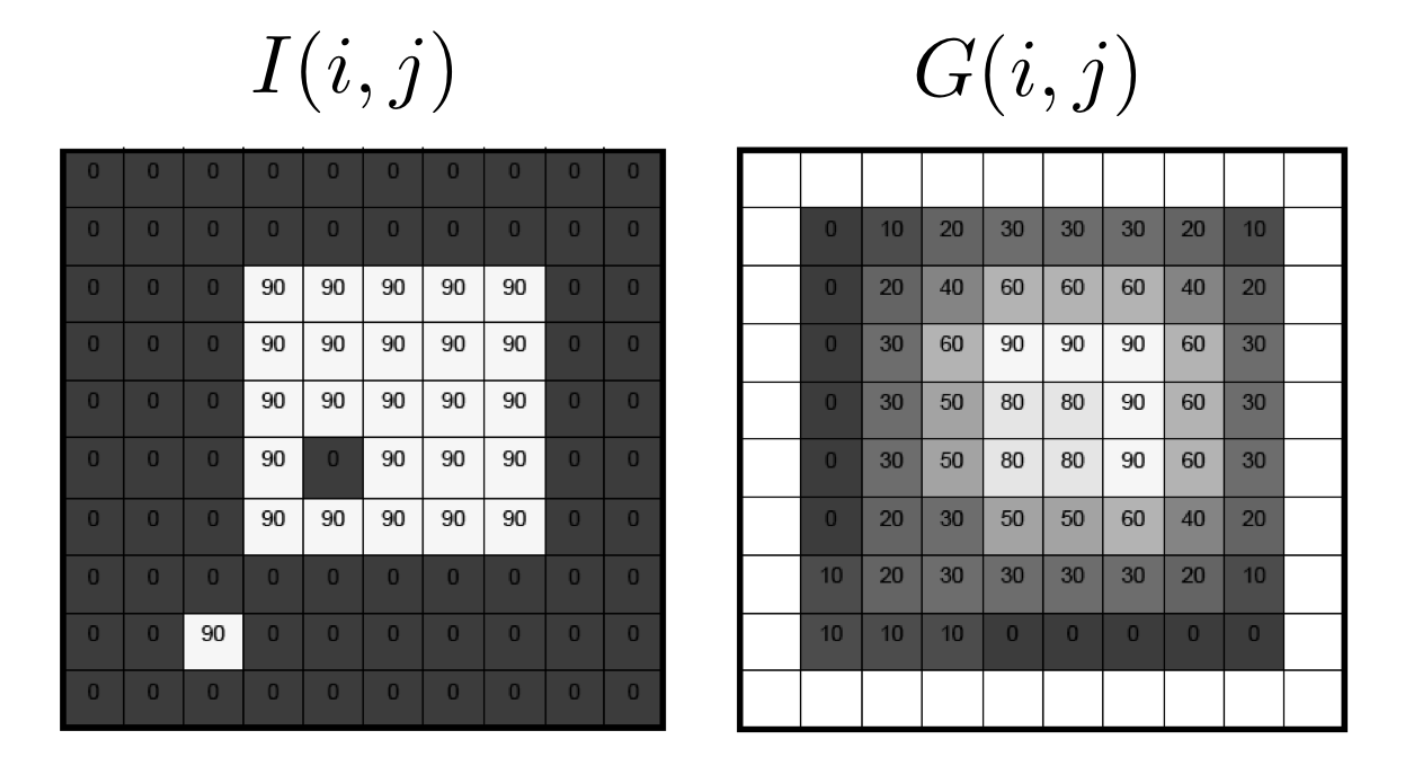
\includegraphics[width=0.6\textwidth]{figs/2dmovingaverage}
	\caption{Example of using moving average to smooth out an image, \textit{assuming no padding}. }
	\label{fig:2dmovingaverage}
\end{figure} 

Much similar to the 1-D case mentioned above, we have our choice of whether to choose an uniform filter or not. 
\begin{itemize}
	\item In the case of uniform (aka moving average), we choose (example of $3 \times 3$ filter)
		\begin{equation}
			\begin{bmatrix}
				1 & 1 & 1 \\
				1 & 1 & 1 \\
				1 & 1 & 1
			\end{bmatrix} / 9
		\end{equation}
	Figure \ref{fig:2dmovingaverage} is an example of using moving average to smooth out an image, \textit{assuming no padding}. Notice that the sharp boundaries that we used to have between dark and white is now smooth. Also, the isolated pixels ($(6, 5)$ and $(9, 3)$) are now blended in. \info{De-noising is usually an important first step (preprocessing) in any image task} 
	\item In case of non-uniform, we can again choose a gaussian like filter, such as
		\begin{equation}
			\begin{bmatrix}
				1 & 4 & 1 \\
				4 & 10 & 4 \\
				1 & 4 & 1
			\end{bmatrix} / 30
		\end{equation}
\end{itemize}

\subsection{Correlation Defined}
\subsubsection{General Moving Average}
In the general case, our filter could be any size. In particular, it needs to be of size square of an odd number. Then, the moving average becomes
\begin{equation}
	G(i, j)=\frac{1}{(2 k+1)^{2}} \sum_{u=-k}^{k} \sum_{v=-k}^{k} I(i+u, j+v)\label{eq:generalmovingaverage}
\end{equation}
\subsubsection{General Filtering}
If we apply some filter (i.e., not just a average) then we can use
\begin{equation}
	G(i, j)=\sum_{u=-k}^{k} \sum_{v=-k}^{k} F(u, v) \cdot I(i+u, j+v)\label{eq:generalfiltering}
\end{equation}
where $F(\cdot, \cdot): \real^2 \rightarrow \real$ is the called \textit{\textbf{kernel}} or \textit{\textbf{mask}} or \textit{\textbf{filter}} such that $\sum_{u'}\sum_{v'}F(u, v) = 1$. The elements of the filter is called \textit{\textbf{filter coefficients}}. Notice that if we take ($|V|, |U|$ here denotes the max values that $v, u$ can take)
\begin{equation}
	F(u, v) = \frac{1}{(2|U| + 1)^{2}} = \frac{1}{(2|V| + 1)^{2}}
\end{equation}
then Equation \ref{eq:generalfiltering} just collapses to Equation \ref{eq:generalmovingaverage}.
\subsubsection{Notation}
The Filtering operation defined above is called \textit{correlation}, denoted as
\begin{equation}
	G = F\otimes I
\end{equation}
where $F$ is our filter / kernel / mask, and $I$ is the original image. \info{Notice that filter is also an image, so $\otimes$ essentially takes two images as input and outputs one image. }

\subsubsection{Correlation - Vector Form}
Define 
\begin{itemize}
	\item $\bf = F(:)$, writing the matrix into a vector.
	\item $T_{i j}=I(i-k: i+k, j-k: j+k)$, the part of image covered by the filter around original image at coordinates $(i, j)$
	\item $\mathbf{t}_{i j}=T_{i j}(:)$ putting the part of image selected in previous step into a vector. 
\end{itemize}
then, 
\begin{equation}
	G(i, j)= \langle \mathbf{f}, \mathbf{t}_{i j}\rangle = \norm{\bf}\norm{\bt_{ij}}\cos \theta
\end{equation}
which converts two for loops into one inner product. This is much faster to compute as far as codes are concerned. 
\unsure{TODO: above we defined correlation for one pixel as a vector operation, can we define the entire correlation into matrix form}
%TODO: above we defined correlation for one pixel as a vector operation, can we define the entire correlation into matrix form?

\subsubsection{Normalized Cross-correlation}
In the task of finding Waldo, we wish to get a score of whether or not a patch of image looks like Waldo. In particular, we want this score to be the highest for the patch with Waldo, but not a very bright patch without Waldo. In an hope to achieve this goal, we can use normalized cross correlation: (utilizing the vector forms in the previous section)
\begin{equation}
	G(i, j)=\frac{\mathbf{f}^\top \mathbf{t}_{i j}}{\|\mathbf{f}\|\left\|\mathbf{t}_{\mathrm{ij}}\right\|} = \cos \theta
\end{equation}
where $\theta$ is the angle between vectors $\bf$ and $\bt_{ij}$

\subsection{Boundary Effects}
Assume we have image size of $m \times n$, and filter size of $k \times k$. Referring to \texttt{cv2.filter2d} in OpenCV and \texttt{filter2(F, I, SHAPE)}, we have the following cases: 
\begin{itemize}
	\item \texttt{shape = `full'} output size is bigger than the image; infinite padding include all reasonable values. Output should have size $(m + 2k - 2) \times ( n + 2k - 2)$
	\item \texttt{shape = `same'} output size is same as $I$; padding such that output size is equal to input size. 
	\item \texttt{shape = `valid'} output size is smaller than the image; no zero padding; output should be size $(n - k + 1) \times (m - k + 1) $
\end{itemize}

\subsection{Smoothing}
\subsubsection{Uniform Smoothing}
\begin{figure}[H]
	\center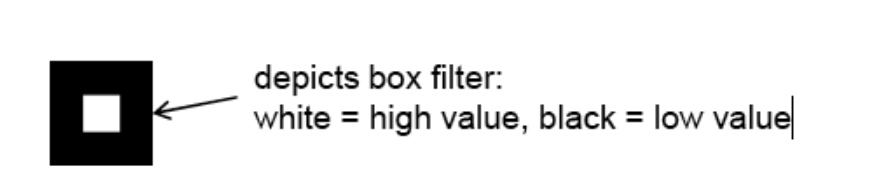
\includegraphics[width=0.6\textwidth]{figs/box_filter}
	\caption{Box Filter}\label{fig:box_filter}
\end{figure}
The box filter depicted in Figure \ref{fig:box_filter} is the exact same filter if we only keep the white part, i.e. the 1 entries. As the size of the box filter increases, the end result gets more and more blurry. 

\subsubsection{Isotropic Gaussian Filter}
\begin{figure}[H]
	\center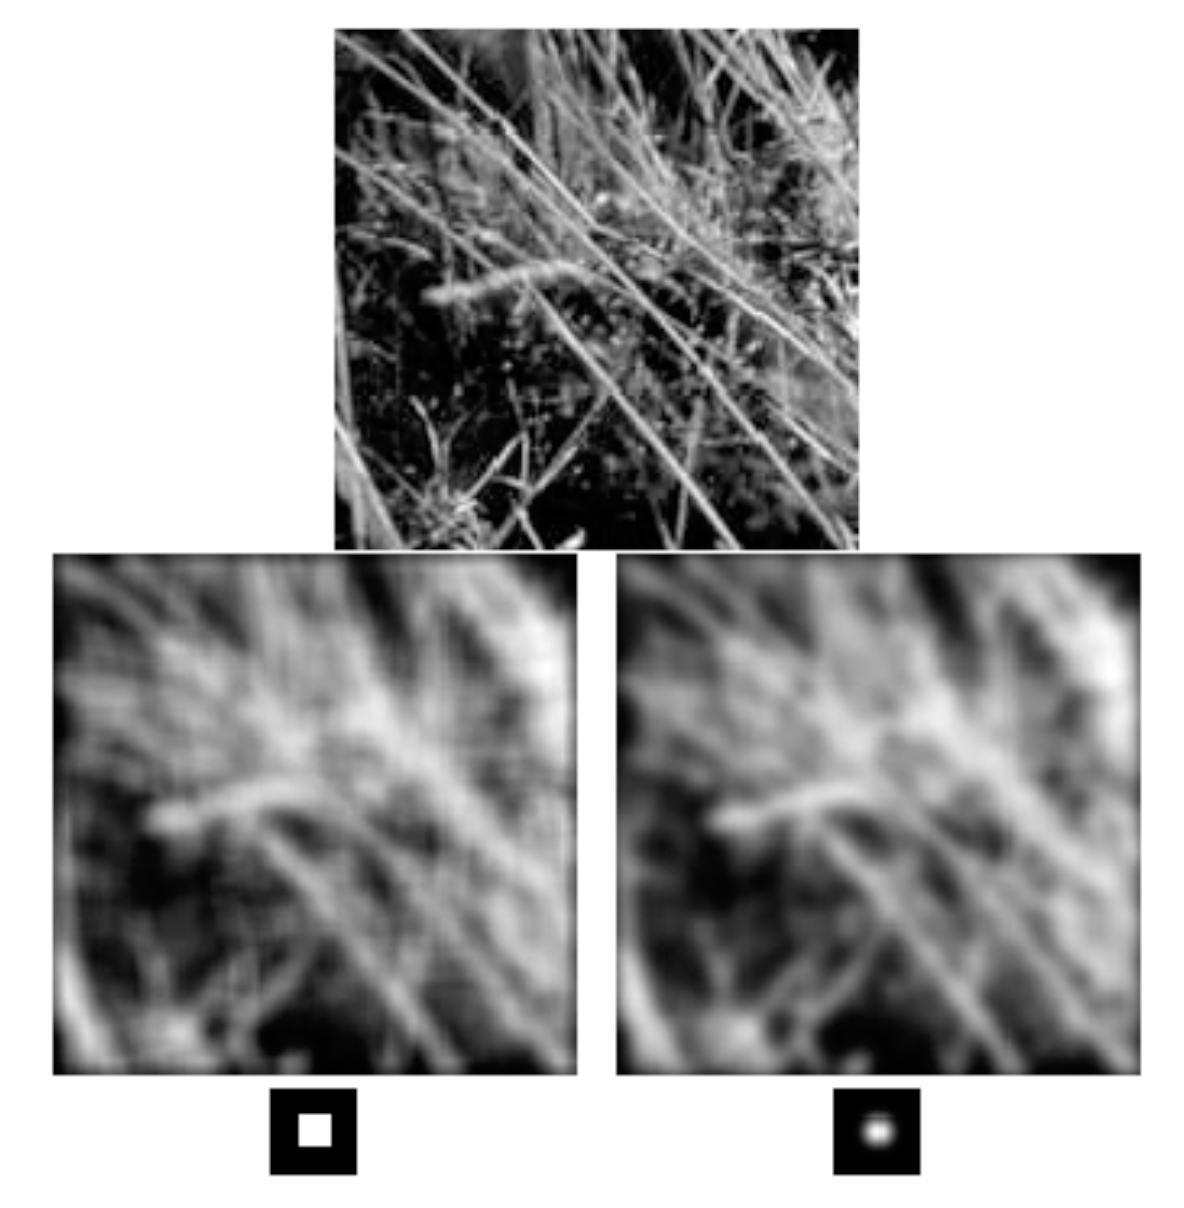
\includegraphics[width=0.6\textwidth]{figs/filter_comp}
	\caption{Comparison of filtered result using uniform filter (bottom left) and gaussian filter (bottom right)}
	\label{fig:filter_comp}
\end{figure}
Recall that the gaussian probability distribution is defined as 
\begin{equation}
	\text{Gaussian}(\bx; \boldsymbol{\mu}, \Sigma ) = (2 \pi)^{-\frac{k}{2}} \operatorname{det}(\Sigma)^{-\frac{1}{2}} e^{-\frac{1}{2}(\mathbf{x}-\boldsymbol{\mu})^{\top} \Sigma^{-1}(\mathbf{x}-\boldsymbol{\mu})}
\end{equation}
and we can mimic this to develop a filter that has entries mimicking values taken by the gaussian pdf. These filters produce results much nice than averaging in terms of smoothing, as we can see in Figure \ref{fig:filter_comp}.

\paragraph{Specification} The Gaussian Filter $G$ is parametrized by two parameters $\Sigma = \sigma I$ (isotropic) and $\boldsymbol{\mu}$. In application, $\boldsymbol{\mu}$ doesn't matter, we always want to make sure that the peak of the gaussian pdf corresponds to the centre pixel of the filter. The size of the filter depends on our choice of $\Sigma$, e.g. it doesn't make much sense if our kernel includes values more than $2\sigma$'s away. We also need to normalize all the taken values again, to make sure the filter we chose sums up to one!

\subsubsection{Non-isotropic Gaussian Filter}
In the most general case, gaussian can be non-isotropic, meaning that its variance-covariance matrix \textit{\textbf{is not}} of form $\sigma I$ 

\subsection{Convolution}
The Convolution operation is defined as
\begin{equation}
	G(i, j)=\sum_{u=-k}^{k} \sum_{v=-k}^{k} F(u, v) \cdot I(i-u, j-v)
	\label{eq:conv}
\end{equation}
Notice that this is exactly the same as Correlation defined in Equation \ref{eq:generalfiltering} except that we are flipping the filter in both dimensions (bottom to top, right to left). \note{In the case of Gaussian / box filters, since the filter will be symmetric about both horizontal and vertical axis, $F \ast I = F \otimes I$.}

\subsubsection{Properties of Convolution}
Convolution is a Linear Operation, meaning that if $f, g$ and $h$ are three convolution operators, and $\lambda \in \real$ then
\begin{itemize}
	\item \textit{\textbf{Commutative}}: $f * g=g * f$
	\item \textit{\textbf{Associative}}: $f *(g * h)=(f * g) * h$
	\item \textit{\textbf{Distributive}}: $f *(g+h)=f * g+f * h$
	\item \textit{\textbf{Assoc. with scalar multiplier}}: $\lambda \cdot(f * g)=(\lambda \cdot f) * g$
\end{itemize}

\subsubsection{Convolution w/ Fourier Transforms}
The Fourier transform of two convolved images is the inner product of their individual Fourier Transforms, i.e.
\begin{equation}
	\mathcal{F}(f * g)= \langle \mathcal{F}(f), \mathcal{F}(g) \rangle
\end{equation}
\paragraph{Implications} The computational complexity of Fourier Transform is much lower than that of convolution. Also notice that inner products are fast to compute. \unsure{Confirm and finish this !}


\subsection{Separable Filters}
For a $K \times K$ sized filter / kernel, the process of performing a convolution requires $K^2$ operations per pixel, summing up to a total of $\#\text{pixels} \times K^2$ for an entire image. In many cases, though not all, we can speed this process up by (1) performing a 1-D horizontal convolution followed by (2) a 1D vertical convolution, requiring only $2K$ operations! When we can do this trick, we call the kernel ``separable''. And a filter is separable iff it is the outer product of two vectors (each a 1D filter):
\begin{equation}
	\exists?\, \bv, \bh \in \real^K, s.t.\,\, F=\mathbf{v} \mathbf{h}^{\top}	
\end{equation}

\subsubsection{Isotropic Gaussian as Separable Filters}
One famous example of separable filter that we are already familiar with is the Gaussian Filter, assuming isotropic variance. In such case the density breaks down into 
\begin{align}
	\text{Gaussian}(x, y; \boldsymbol \mu = \bzero, \Sigma = \sigma I) 
	&= \frac{1}{2 \pi \sigma^{2}} \exp \left\{-\frac{x^{2}+y^{2}}{\sigma^{2}}\right\} \\
	&= \left[\frac{1}{\sqrt{2 \pi} \sigma} \exp\left\{-\frac{x^{2}}{\sigma^{2}}\right\}\right] \cdot\left[\frac{1}{\sqrt{2 \pi} \sigma} \exp\left\{-\frac{y^{2}}{\sigma^{2}}\right\}\right]
\end{align}
Such factorization of gaussian pdf indicates us that we should have two 1-D filters that are 1-D gaussian each. 

\subsubsection{Moving Average as Separable Filters}
The na\"ive moving average filter that we encountered earlier is also separable, in which case
\begin{equation}
	F = \begin{bmatrix}
		1 & \hdots & 1 \\
		\vdots & \ddots & \vdots \\
		1 & \hdots & 1
	\end{bmatrix} / K^2 = \begin{bmatrix}
		1/K & \dots & 1/K
	\end{bmatrix}^\top  \begin{bmatrix}
		1/K & \dots & 1/K
	\end{bmatrix}
\end{equation}

\subsubsection{Edge Detector Kernel as Separable Filters}
The edge detector \unsure{Come back: left or right edge detector?}
\begin{equation}
	F = \begin{bmatrix}
		-1 & 0 & 1 \\
		-2 & 0 & 2 \\
		-1 & 0 & 1
	\end{bmatrix} / 8; \quad \bv = \begin{bmatrix}
		-1 & 0 & 1
	\end{bmatrix} / 2; \quad F = \bv^\top \bv
\end{equation}

\subsubsection{Separable-ness of Filters}
A systematic way of checking if a kernel is separable if by looking at the singular value decomposition of the filter. \textit{\textbf{If only one singular value is non-zero, the it is separable}}
\begin{equation}
	F=\mathbf{U} \Sigma \mathbf{V}^{\top}=\sum_{i} \sigma_{i} u_{i} v_{i}^{\top}
\end{equation}
with $\Sigma=\operatorname{diag}\left(\sigma_{i}\right)$. Then, we can get the vertical and horizontal filter through
\begin{equation}
	F_\text{vertical} \gets \sqrt{\sigma_{1}} \mathbf{u}_{1} \quad\quad F_\text{horizontal} \gets \sqrt{\sigma_{1}} \mathbf{v}_{1}^{\top }
\end{equation}


\section{Edge Detection}






































\end{document}
